% example.tex
\documentclass[dvisvgm]{standalone}

\usepackage{amsmath}
\usepackage[usenames,dvipsnames]{xcolor}
\usepackage{tikz}
\usetikzlibrary {arrows.meta,
                 calc,
                 positioning,
                 shapes.geometric}

 \tikzset{
        base/.style={draw, align=center, minimum height=4ex},
        proc/.style={base, rectangle, text width=8em},
        io/.style={trapezium, trapezium left angle=70, trapezium right
                   angle=110, draw, text width=8em, %minimum width=2cm, 
                   %minimum height=1cm
                   },
        test/.style={base, diamond, aspect=2,
                     text width=8em
                     },
        term/.style={proc, rounded corners},
        myarrow/.style={-Stealth, line width=0.25mm},
 }

\begin{document}
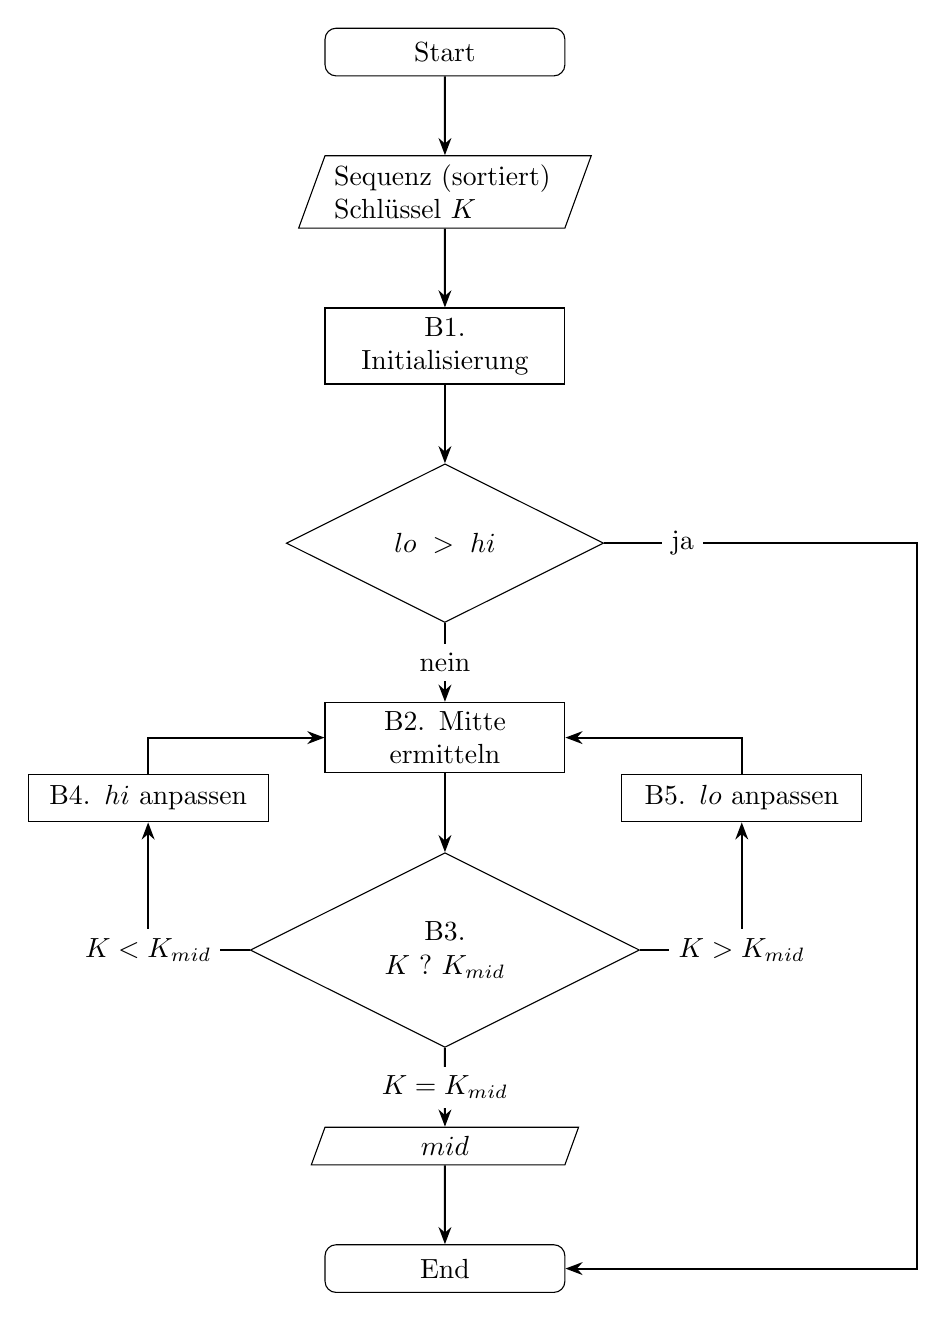
\begin{tikzpicture}
    \node[draw, term] (a) {Start};
    \node[draw, io, below= of a] (b) {Sequenz (sortiert) \linebreak
                                      Schlüssel $K$};
    \node[draw, proc, below= of b] (c) {B1. \linebreak Initialisierung};
    \node[draw, test, below= of c] (d) {$lo > hi$};
    \node[draw, proc, below= of d] (e) {B2. Mitte ermitteln};
    \node[draw, test, below= of e] (f) {B3. \linebreak
          $K\ ?\ K_{mid}$};

    \node[draw, align=center, io, below= of f] (g) {$mid$};
    \node[draw, term, below= of g] (h) {End};

    \node[draw, proc, above left= of f] (i) {B4. $hi$ anpassen};
    \node[draw, proc, above right= of f] (j) {B5. $lo$ anpassen};

    \draw[myarrow] (a) edge (b);
    \draw[myarrow] (b) edge (c);
    \draw[myarrow] (c) edge (d);
    \draw[myarrow] (e) edge (f);
    \draw[myarrow] (g) edge (h);

    \draw[myarrow] (d) edge node[fill=white] {nein} (e);
    \draw[myarrow] (f) edge node[fill=white] {$K = K_{mid}$} (g);
    \draw[myarrow] (f) -| node[fill=white] {$K < K_{mid}$}(i);
    \draw[myarrow] (f) -| node[fill=white] {$K > K_{mid}$} (j);

    \draw[myarrow] (i) |- (e);
    \draw[myarrow] (j) |- (e);

    \draw[myarrow] (d) -| node[very near start, fill=white] {ja} ++(6,0) |-  (h);

    
%    \draw[myarrow] (e.west) -| ++(-.5,0) |- (d.north west);
%    \draw[myarrow] (f.east) -| ++(.5,0) |- (d.north east);
%    \draw[myarrow] (e) -| (g.north);
%    \draw[myarrow] (f) -| (g.north);
%    \draw[myarrow] (g) -| (h);
%    \draw[myarrow] (g) -| (i);

\end{tikzpicture}
\end{document}
